\documentclass[a4paper,12pt]{article}

% Packages
\usepackage{ctex}

\usepackage{amsmath}  % For math formulas
\usepackage{amssymb}  % For additional math symbols
\usepackage{amsfonts} % For more math fonts

\usepackage{geometry} % For adjusting page margins
\geometry{margin=1in} % 1 inch margins

\usepackage{hyperref} % \pdfbookmark dependent on the package

\usepackage{enumitem}

\setlength{\parindent}{0pt}

\usepackage{mdframed}

\usepackage{setspace}
\setstretch{1.25}

\usepackage{multicol}

\usepackage{tikz}

\usepackage{etoolbox}
\usepackage{comment}

\newbool{showDetailedAnswers}

\booltrue{showDetailedAnswers}
%\boolfalse{showDetailedAnswers}

% In addtion of \small, there are some others: \tiny, \scriptsize, \footnotesize, \small, \normalsize, \large, \Large, \LARGE, \huge, \Huge
\newcommand{\detailedAnswers}[1]{%
  \ifbool{showDetailedAnswers}{\par\footnotesize\quad\;\:\textbf{解析}\par #1}{}
}

\begin{document}

% Title Page
\pdfbookmark[0]{Cover}{cover}

\begin{titlepage}
\title{数学奥林匹克小丛书\;第三版\\初中卷 1 因式分解技巧}
\maketitle
\end{titlepage}

% Table of Contents
\pdfbookmark[0]{Contents}{contents}
\tableofcontents
\newpage

\section{提公因式}

\begin{multicols}{2}
\begin{enumerate}
\item $5 x ^ { 2 } y - 1 0 x y z + 5 x y .$

\item $a ( x - a ) + b ( a - x ) - ( x - a ) .$

\item $- 2 x ( x + 1 ) + a ( x + 1 ) + ( x + 1 ) .$

\item ${ \frac { 3 } { 2 } } b ^ { 3 n - 1 } + { \frac { 1 } { 6 } } b ^ { 2 n - 1 }$ (n是正整数).

\item $2 ( p - 1 ) ^ { 2 } - 4 q ( p - 1 ) .$

\item $m n ( m ^ { 2 } + n ^ { 2 } ) - n ^ { 2 } ( m ^ { 2 } + n ^ { 2 } ) .$

\item $( 5 a - 2 b ) ( 2 m + 3 p ) - ( 2 a - 7 b ) ( 2 m + 3p ) .$

\item $2 ( x + y ) + 6 ( x + y ) ^ { 2 } - 4 ( x + y ) ^ { 3 } .$

\item $( x + y ) ^ { 2 } ( b + c ) - ( x + y ) ( b + c ) ^ { 2 } .$

\item $6 p ( x - 1 ) ^ { 3 } - 8 p ^ { 2 } ( x - 1 ) ^ { 2 } - 2 p ( 1 - x ) ^ { 2 } .$
\end{enumerate}
\end{multicols}

\detailedAnswers{
\begin{multicols}{2}
\begin{enumerate}
	\item 原式$ = 5 x y ( x - 2 z + 1 )$.
	
	\item 原式$ = a ( x - a ) - b ( x - a ) - ( x - a ) \\ = ( x - a ) ( a - b - 1 )$.
	
	\item 原式$ = ( x + 1 ) ( - 2 x + a + 1 )$.
	
	\item 原式$ = { \frac { 1 } { 6 } } b ^ { 2 n - 1 } ( 9 b ^ { n } + 1 )$.
	%5
	\item 原式$ = 2 ( p - 1 ) ( p - 1 - 2 q )$.
	
	\item 原式$ = n ( m ^ { 2 } + n ^ { 2 } ) ( m - n )$.
	
	\item 原式$ = ( 2 m + 3 p ) ( 5 a - 2 b - 2 a + 7 b ) \\ = ( 2 m + 3 p ) ( 3 a + 5 b )$.
	%8
	\item 原式$ = 2 ( x + y ) [ 1 + 3 ( x + y ) - 2 ( x + y ) ^ { 2 } ] \\ = 2 ( x + y ) ( 1 + 3 x + 3 y - 2 x ^ { 2 } - 4 x y - 2 y ^ { 2 } )$.
	
	\item 原式$ = ( x + y ) ( b + c ) ( x + y - b - c )$.
	
	\item 原式$ = 2 p ( x - 1 ) ^ { 2 } [ 3 ( x - 1 ) - 4 p - 1 ]$.
\end{enumerate}
\end{multicols}
}

\section{应用公式}

\begin{multicols}{2}
\begin{enumerate}
\item $1 6 - ( 3 a + 2 b ) ^ { 2 } .$

\item $4 y ^ { 2 } - ( 2 z - x ) ^ { 2 } .$

\item $a ^ { 4 } - b ^ { 4 } .$

\item $- 8 1 a ^ { 4 } b ^ { 4 } + 1 6 c ^ { 4 } .$

\item $2 0 a ^ { 3 } x ^ { 3 } - 4 5 a x y ^ { 2 } .$

\item $( 3 a ^ { 2 } - b ^ { 2 } ) ^ { 2 } - ( a ^ { 2 } - 3 b ^ { 2 } ) ^ { 2 } .$

\item $x ^ { 8 } - y ^ { 8 } .$

\item $1 6 x ^ { 5 } - x .$

\item $( 5 x ^ { 2 } + 2 x - 3 ) ^ { 2 } - ( x ^ { 2 } - 2 x - 3 ) ^ { 2 } .$

\item $3 2 a ^ { 3 } b ^ { 3 } \! - \! 4 b ^ { 9 } .$

\item $8 a ^ { 3 } b ^ { 3 } c ^ { 3 } - 1 .$

\item $6 4 x ^ { 6 } y ^ { 3 } + y ^ { 1 5 } .$

\item $x ^ { 2 } ( a + b ) ^ { 2 } - 2 x y ( a ^ { 2 } - b ^ { 2 } ) + y ^ { 2 } ( a - b ) ^ { 2 } .$

\item $a ^ { n + 2 } + 8 a ^ { n } + 1 6 a ^ { n - 2 } . $

\item $9 a ^ { 2 } + x ^ { 2 n } + 6 a + 2 x ^ { n } + 6 a x ^ { n } + 1 .$

\item $a ^ { 2 } + b ^ { 2 } + c ^ { 2 } + 2 a b - 2 a c - 2 b c .$

\item $ x ^ { 2 } + 9 y ^ { 2 } + 4 z ^ { 2 } - 6 x y + 4 x z - 1 2 y z .$

\item $( p + q ) ^ { 3 } - 3 ( p + q ) ^ { 2 } ( p - q ) + 3 ( p + q ) ( p - q ) ^ { 2 } - ( p - q ) ^ { 3 } .$

\item $ 4 a ^ { 2 } b ^ { 2 } - ( a ^ { 2 } + b ^ { 2 } ) ^ { 2 } .$

\item $( a + x ) ^ { 4 } - ( a - x ) ^ { 4 } .$
\end{enumerate}
\end{multicols}

\detailedAnswers{
\begin{multicols}{2}
\begin{enumerate}
	\item 原式$=4 ^ { 2 } - ( 3 a + 2 b ) ^ { 2 } \\ = ( 4 + 3 a + 2 b ) ( 4 - 3 a - 2 b )$.
	
	\item 原式$=( 2 y ) ^ { 2 } - ( 2 z - x ) ^ { 2 } \\ = ( 2 y + 2 z - x ) ( 2 y - 2 z + x )$.
	
	\item 原式$=( a ^ { 2 } ) ^ { 2 } - ( b ^ { 2 } ) ^ { 2 } \\ = ( a ^ { 2 } + b ^ { 2 } ) ( a ^ { 2 } - b ^ { 2 } ) \\ =( a ^ { 2 } + b ^ { 2 } ) ( a + b ) ( a - b ) $.
	
	\item 原式$=( 4 c ^ { 2 } ) ^ { 2 } - ( 9 a ^ { 2 } b ^ { 2 } ) ^ { 2 } \\ = ( 4 c ^ { 2 } + 9 a ^ { 2 } b ^ { 2 } ) ( 4 c ^ { 2 } - 9 a ^ { 2 } b ^ { 2 } ) \\ = ( 4 c ^ { 2 } + 9 a ^ { 2 } b ^ { 2 } ) ( 2 c + 3 a b ) ( 2 c - 3 a b )$.
	
	%5
	\item 原式$=5 a x ( 4 a ^ { 2 } x ^ { 2 } - 9 y ^ { 2 } ) \\ = 5 a x ( 2 a x + 3 y ) ( 2 a x - 3 y )$.
	
	\item 原式$=( 3 a ^ { 2 } - b ^ { 2 } + a ^ { 2 } - 3 b ^ { 2 } ) ( 3 a ^ { 2 } - b ^ { 2 } - a ^ { 2 } + 3 b ^ { 2 } ) \\ = ( 4 a ^ { 2 } - 4 b ^ { 2 } ) ( 2 a ^ { 2 } + 2 b ^ { 2 } ) \\ = 8 ( a + b ) ( a - b ) ( a ^ { 2 } + b ^ { 2 } )$.
	
	\item 原式$=( x ^ { 4 } ) ^ { 2 } - ( y ^ { 4 } ) ^ { 2 } \\ = ( x ^ { 4 } + y ^ { 4 } ) ( x ^ { 4 } - y ^ { 4 } ) \\ = ( x ^ { 4 } + y ^ { 4 } ) ( x ^ { 2 } + y ^ { 2 } ) ( x + y ) ( x - y )$.
	
	(利用第3题的结果)
	
	%8
	\item 原式$=x ( 1 6 x ^ { 4 } - 1 ) \\ = x [ ( 2 x ) ^ { 4 } - 1 ^ { 4 } ] \\ = x [ ( 2 x ) ^ { 2 } + 1 ] ( 2 x + 1 ) ( 2 x - 1 ) \\ = x ( 4 x ^ { 2 } + 1 ) ( 2 x + 1 ) ( 2 x - 1 )$.
	
	\item 原式$=( 5 x ^ { 2 } + 2 x - 3 + x ^ { 2 } - 2 x - 3 ) ( 5 x ^ { 2 } + 2 x - 3 - x ^ { 2 } + 2 x + 3 ) \\ = ( 6 x ^ { 2 } - 6 ) ( 4 x ^ { 2 } + 4 x ) \\ = 2 4 x ( x ^ { 2 } - 1 ) ( x + 1 ) \\ = 2 4 x ( x - 1 ) ( x + 1 ) ^ { 2 }$.
	
	\item 原式$=4 b ^ { 3 } ( 8 a ^ { 3 } - b ^ { 6 } ) = 4 b ^ { 3 } [ ( 2 a ) ^ { 3 } - ( b ^ { 2 } ) ^ { 3 } ] \\ = 4 b ^ { 3 } ( 2 a - b ^ { 2 } ) [ ( 2 a ) ^ { 2 } + 2 a b ^ { 2 } + ( b ^ { 2 } ) ^ { 2 } ] \\ = 4 b ^ { 3 } ( 2 a - b ^ { 2 } ) ( 4 a ^ { 2 } + 2 a b ^ { 2 } + b ^ { 4 } )$.
	
	\item 原式$=( 2 a b c ) ^ { 3 } - 1 ^ { 3 } \\ = ( 2 a b c - 1 ) ( 4 a ^ { 2 } b ^ { 2 } c ^ { 2 } + 2 a b c + 1 )$.
	
	%12
	\item 原式$=y ^ { 3 } ( 6 4 x ^ { 6 } + y ^ { 1 2 } ) \\ = y ^ { 3 } [ ( 4 x ^ { 2 } ) ^ { 3 } + ( y ^ { 4 } ) ^ { 3 } ] \\ = y ^ { 3 } ( 4 x ^ { 2 } + y ^ { 4 } ) ( 1 6 x ^ { 4 } - 4 x ^ { 2 } y ^ { 4 } + y ^ { 8 } )$.
	
	\item 原式$=[ x ( a + b ) ] ^ { 2 } - 2 x ( a + b ) \cdot y ( a - b ) + [ y ( a - b ) ] ^ { 2 } \\ = [ x ( a + b ) - y ( a - b ) ] ^ { 2 } \\ = ( a x + b x - a y + b y ) ^ { 2 }$.
	
	\item 原式$=a ^ { n - 2 } ( a ^ { 4 } + 8 a ^ { 2 } + 1 6 ) \\ = a ^ { n - 2 } [ ( a ^ { 2 } ) ^ { 2 } + 2 \times 4 \times a ^ { 2 } + 4 ^ { 2 } ] \\ = a ^ { n - 2 } ( a ^ { 2 } + 4 ) ^ { 2 }$.
	
	%15
	\item 原式$=( x ^ { 2 n } + 2 x ^ { n } + 1 ) + 6 a ( x ^ { n } + 1 ) + 9 a ^ { 2 } \\ = ( x ^ { n } + 1 ) ^ { 2 } + 6 a ( x ^ { n } + 1 ) + ( 3 a ) ^ { 2 } \\ = ( x ^ { n } + 1 + 3 a ) ^ { 2 }$.
	
	\item 原式$=( a ^ { 2 } + 2 a b + b ^ { 2 } ) - 2 c ( a + b ) + c ^ { 2 } \\ = ( a + b ) ^ { 2 } - 2 c ( a + b ) + c ^ { 2 } \\ = ( a + b - c ) ^ { 2 }$.
	
	\item 原式$=( x ^ { 2 } - 6 x y + 9 y ^ { 2 } ) + 4 z ( x - 3 y ) + 4 z ^ { 2 } \\ = ( x - 3 y ) ^ { 2 } + 4 z ( x - 3 y ) + ( 2 z ) ^ { 2 } \\ = ( x - 3 y + 2 z ) ^ { 2 }$.
	
	%18
	\item 原式$=[ ( p + q ) - ( p - q ) ] ^ { 3 } = = ( 2 q ) ^ { 3 } \\ = 8q^3 $.
	
	\item 原式$=( 2 a b + a ^ { 2 } + b ^ { 2 } ) ( 2 a b - a ^ { 2 } - b ^ { 2 } ) \\ = - ( a ^ { 2 } + 2 a b + b ^ { 2 } ) ( a ^ { 2 } - 2 a b + b ^ { 2 } ) \\ = - ( a + b ) ^ { 2 } ( a - b ) ^ { 2 }$.
	
	\item 原式$=[ ( a + x ) ^ { 2 } + ( a - x ) ^ { 2 } ] [ ( a + x ) ^ { 2 } - ( a - x ) ^ { 2 } ] \\ = ( a ^ { 2 } + 2 a x + x ^ { 2 } + a ^ { 2 } - 2 a x + x ^ { 2 } ) ( a + x + a - x ) ( a + x - a + x ) \\ = 8 a x ( a ^ { 2 } + x ^ { 2 } )$.
\end{enumerate}
\end{multicols}
}

\section{分组分解}

\begin{multicols}{2}
\begin{enumerate}
\item $a x - a y + b x + c y - c x - b y .$

\item $x ^ { 4 } + x ^ { 3 } + x ^ { 2 } - 1 .$

\item $a ( 1 - b + b ^ { 2 } ) - 1 + b - b ^ { 2 } .$

\item $4 x ( a ^ { 2 } + x ^ { 2 } ) - a ^ { 2 } - x ^ { 2 } .$
% 5
\item $a b x ^ { 2 } + b x y - a x y - y ^ { 2 } .$

\item $a ^ { 2 } b ^ { 3 } - a b c ^ { 2 } d + a b ^ { 2 } c d - c ^ { 3 } d ^ { 2 } .$

\item $3 2 a c ^ { 2 } + 1 5 c x ^ { 2 } - 4 8 a x ^ { 2 } - 1 0 c ^ { 3 } .$

\item $2 ( x ^ { 2 } - 3 a b ) + x ( 4 a - 3 b ) .$

\item $x ^ { 3 } - x + y ^ { 3 } - y .$

% 10
\item $x ^ { 3 } + y ^ { 3 } + x ^ { 2 } + 2 x y + y ^ { 2 } .$

\item $4 a ^ { 2 } - b ^ { 2 } + c ^ { 2 } - 9 d ^ { 2 } + 4 a c + 6 b d .$

\item $a ( 1 - b ) ^ { 2 } - 1 + 2 b - b ^ { 2 } .$

\item $x ( x + z ) - y ( y + z ) .$

\item $x ^ { 3 } + b x ^ { 2 } + a x + a b .$

% 15

\item $a c x ^ { 3 } + b c x ^ { 2 } + a d x + b d .$

\item $a ^ { 4 } + a ^ { 3 } b - a b ^ { 3 } - b ^ { 4 } .$

\item $a ^ { 4 } - a ^ { 3 } b - a b ^ { 3 } + b ^ { 4 } .$

\item $a ^ { 2 } b ^ { 2 } - a ^ { 2 } - b ^ { 2 } + 1 .$

\item $x ^ { 2 } y ^ { 2 } - x ^ { 2 } z ^ { 2 } - y ^ { 2 } z ^ { 2 } + z ^ { 4 } .$

% 20
\item $x ^ { 2 } y ^ { 2 } z ^ { 2 } - x ^ { 2 } z - y ^ { 2 } z + 1 .$

\item $x ^ { 4 } + x ^ { 3 } y + x z ^ { 3 } + y z ^ { 3 } .$

\item $( a + b ) ^ { 2 } + ( a + c ) ^ { 2 } - ( c + d ) ^ { 2 } - ( b + d ) ^ { 2 } .$

\item $a x ( y ^ { 3 } + b ^ { 3 } ) + b y ( b x ^ { 2 } + a ^ { 2 } y ) .$

\item $( a + b ) ^ { 3 } + ( b + c ) ^ { 3 } + ( c + a ) ^ { 3 } + a ^ { 3 } + b ^ { 3 } + c ^ { 3 } .$
\end{enumerate}
\end{multicols}

\detailedAnswers{
\begin{enumerate}
\begin{multicols}{2}
\item 原式$ = ( a x + b x - c x ) - ( a y + b y - c y ) \\ = x ( a + b - c ) - y ( a + b - c ) \\ = ( x - y ) ( a + b - c ) . $

\item 原式$ = ( x ^ { 4 } + x ^ { 3 } ) + ( x ^ { 2 } - 1 ) \\ = x ^ { 3 } ( x + 1 ) + ( x + 1 ) ( x - 1 ) \\ = ( x + 1 ) ( x ^ { 3 } + x - 1 ) . $

\item 原式$ = a ( 1 - b + b ^ { 2 } ) - ( 1 - b + b ^ { 2 } ) \\ = ( a - 1 ) ( 1 - b + b ^ { 2 } ) . $

\item 原式$ = 4 x ( a ^ { 2 } + x ^ { 2 } ) - ( a ^ { 2 } + x ^ { 2 } ) \\ = ( a ^ { 2 } + x ^ { 2 } ) ( 4 x - 1 ) . $

% 5
\item 原式$ = ( a b x ^ { 2 } + b x y ) - ( a x y + y ^ { 2 } ) \\ = b x ( a x + y ) - y ( a x + y ) \\ = ( a x + y ) ( b x - y ) .$

或\ 原式$= ( a b x ^ { 2 } - a x y ) + ( b x y - y ^ { 2 } ) \\ = a x ( b x - y ) + y ( b x - y ) \\ = ( b x - y ) ( a x + y ) .$

% 6
\item 原式$= ( a ^ { 2 } b ^ { 3 } - a b c ^ { 2 } d ) + ( a b ^ { 2 } c d - c ^ { 3 } d ^ { 2 } ) \\ = a b ( a b ^ { 2 } - c ^ { 2 } d ) + c d ( a b ^ { 2 } - c ^ { 2 } d ) \\ = ( a b ^ { 2 } - c ^ { 2 } d ) ( a b + c d ) . $

% 7
\item 原式 $= ( 3 2 a c ^ { 2 } - 4 8 a x ^ { 2 } ) + ( 1 5 c x ^ { 2 } - 1 0 c ^ { 3 } ) \\ = 1 6 a ( 2 c ^ { 2 } - 3 x ^ { 2 } ) + 5 c ( 3 x ^ { 2 } - 2 c ^ { 2 } ) \\ = ( 2 c ^ { 2 } - 3 x ^ { 2 } ) ( 1 6 a - 5 c ) . \\ $
或\ 原式$ = ( 3 2 a c ^ { 2 } - 1 0 c ^ { 3 } ) + ( 1 5 c x ^ { 2 } - 4 8 a x ^ { 2 } ) \\ = 2 c ^ { 2 } ( 1 6 a - 5 c ) + 3 x ^ { 2 } ( 5 c - 1 6 a ) \\ = ( 1 6 a - 5 c ) ( 2 c ^ { 2 } - 3 x ^ { 2 } ) . $

% 8
\item 原式$ = 2 x ^ { 2 } - 6 a b + 4 a x - 3 b x \\ = ( 2 x ^ { 2 } + 4 a x ) - ( 6 a b + 3 b x ) \\ = 2 x ( x + 2 a ) - 3 b ( 2 a + x ) \\ = ( x + 2 a ) ( 2 x - 3 b ) . \\ $
或\ 原式$= 2 x ^ { 2 } - 6 a b + 4 a x - 3 b x \\ = ( 2 x ^ { 2 } - 3 b x ) + ( 4 a x - 6 a b ) \\ \text{(正项放在负项前面较好)} \\ = x ( 2 x - 3 b ) + 2 a ( 2 x - 3 b ) \\ = ( 2 x - 3 b ) ( x + 2 a ) .$

% 9
\item 原式$= ( x ^ { 3 } + y ^ { 3 } ) - ( x + y ) \\ = ( x + y ) ( x ^ { 2 } - x y + y ^ { 2 } ) - ( x + y ) \\ = ( x + y ) ( x ^ { 2 } - x y + y ^ { 2 } - 1 ) .$

% 10
\item 原式$ = ( x ^ { 3 } + y ^ { 3 } ) + ( x ^ { 2 } + 2 x y + y ^ { 2 } ) \\ = ( x + y ) ( x ^ { 2 } - x y + y ^ { 2 } ) + ( x + y ) ^ { 2 } \\ = ( x + y ) ( x ^ { 2 } - x y + y ^ { 2 } + x + y ) .$

\item 原式$= ( 4 a ^ { 2 } + c ^ { 2 } + 4 a c ) - ( b ^ { 2 } - 6 b d + 9 d ^ { 2 } ) \\ = ( 2 a + c ) ^ { 2 } - ( b - 3 d ) ^ { 2 } \\ = ( 2 a + c + b - 3 d ) ( 2 a + c - b + 3 d ) .$

(因为有$4 a c$,所以将含$ a $或$ c $的项放在一起.同样,将含$ b $或$ d $的项放在一起)

% 12
\item 原式$ = a ( 1 - b ) ^ { 2 } - ( 1 - 2 b + b ^ { 2 } ) \\ = a ( 1 - b ) ^ { 2 } - ( 1 - b ) ^ { 2 } \\ = ( 1 - b ) ^ { 2 } ( a - 1 ) .$

\item 原式$= x ^ { 2 } + x z - y ^ { 2 } - y z\\ = ( x ^ { 2 } - y ^ { 2 } ) + ( x z - y z )\\ = ( x + y ) ( x - y ) + z ( x - y )\\ = ( x - y ) ( x + y + z ) .$

\item 原式$= ( x ^ { 3 } + b x ^ { 2 } ) + ( a x + a b )\\ = x ^ { 2 } ( x + b ) + a ( x + b )\\ = ( x + b ) ( x ^ { 2 } + a ) .$

% 15
\item 原式$= ( a x ^ { 3 } + b c x ^ { 2 } ) + ( a d x + b d )\\ = c x ^ { 2 } ( a x + b ) + d ( a x + b )\\ = ( a x + b ) ( c x ^ { 2 } + d ).$

\item 原式$ = ( a ^ { 4 } - a ^ { 3 } b ) - ( a b ^ { 3 } - b ^ { 4 } ) \\ = a ^ { 3 } ( a - b ) - b ^ { 3 } ( a - b ) \\ = ( a - b ) ( a ^ { 3 } - b ^ { 3 } ) \\ = ( a - b ) ^ { 2 } ( a ^ { 2 } + a b + b ^ { 2 } ) .$

\item 原式$=( a ^ { 4 } - a ^ { 3 } b ) - ( a b ^ { 3 } - b ^ { 4 } ) \\ = a ^ { 3 } ( a - b ) - b ^ { 3 } ( a - b ) \\ = ( a - b ) ( a ^ { 3 } - b ^ { 3 } ) \\ = ( a - b ) ^ { 2 } ( a ^ { 2 } + a b + b ^ { 2 } )$.

%18
\item 原式$( a ^ { 2 } b ^ { 2 } - a ^ { 2 } ) - ( b ^ { 2 } - 1 ) \\ = a ^ { 2 } ( b ^ { 2 } - 1 ) - ( b ^ { 2 } - 1 ) \\ = ( b ^ { 2 } - 1 ) ( a ^ { 2 } - 1 )  \\ = ( a + 1 ) ( a - 1 ) ( b + 1 ) ( b - 1 )$.

\item 原式$=( x ^ { 2 } y ^ { 2 } - x ^ { 2 } z ^ { 2 } ) - ( y ^ { 2 } z ^ { 2 } - z ^ { 4 } ) \\ = x ^ { 2 } ( y ^ { 2 } - z ^ { 2 } ) - z ^ { 2 } ( y ^ { 2 } - z ^ { 2 } ) \\ = ( y ^ { 2 } - z ^ { 2 } ) ( x ^ { 2 } - z ^ { 2 } ) \\ = ( x + z ) ( x - z ) ( y + z ) ( y - z )$.

%20
\item 原式$=( x ^ { 2 } y ^ { 2 } z ^ { 2 } - x ^ { 2 } z ) - ( y ^ { 2 } z - 1 ) \\ = x ^ { 2 } z ( y ^ { 2 } z - 1 ) - ( y ^ { 2 } z - 1 ) \\ = ( y ^ { 2 } z - 1 ) ( x ^ { 2 } z - 1 )$.

\item 原式$=( x ^ { 4 } + x ^ { 3 } y ) + ( x z ^ { 3 } + y z ^ { 3 } ) \\ = x ^ { 3 } ( x + y ) + z ^ { 3 } ( x + y ) \\ = ( x + y ) ( x ^ { 3 } + z ^ { 3 } ) \\ = ( x + y ) ( x + z ) ( x ^ { 2 } - x z + z ^ { 2 } )$.

\item 原式$=[ ( a + b ) ^ { 2 } - ( c + d ) ^ { 2 } ] + [ ( a + c ) ^ { 2 } - ( b + d ) ^ { 2 } ] \\ = ( a + b + c + d ) ( a + b - c - d ) \\ + ( a + c + b + d ) ( a + c - b - d ) \\ = ( a + b + c + d ) ( 2 a - 2 d ) \\ = 2 ( a + b + c + d ) ( a - d )$.

或\:原式$=[ ( a + b ) ^ { 2 } - ( b + d ) ^ { 2 } ] + [ ( a + c ) ^ { 2 } - ( c + d ) ^ { 2 } ] \\ = ( a + 2 b + d ) ( a - d ) + ( a + 2 c + d ) ( a - d ) \\ = ( a - d ) ( 2 a + 2 b + 2 c + 2 d ) \\ = 2 ( a - d ) ( a + b + c + d )$.

%23
\item 原式$=a x y ^ { 3 } + a b ^ { 3 } x + b ^ { 2 } x ^ { 2 } y + a ^ { 2 } b y ^ { 2 } \\ = ( a x y ^ { 3 } + b ^ { 2 } x ^ { 2 } y ) + ( a b ^ { 3 } x + a ^ { 2 } b y ^ { 2 } ) \\ = x y ( a y ^ { 2 } + b ^ { 2 } x ) + a b ( b ^ { 2 } x + a y ^ { 2 } ) \\ = ( a y ^ { 2 } + b ^ { 2 } x ) ( x y + a b )$.

或\:原式$=a x y ^ { 3 } + a b ^ { 3 } x + b ^ { 2 } x ^ { 2 } y + a ^ { 2 } b y ^ { 2 } \\ = ( a x y ^ { 3 } + a ^ { 2 } b y ^ { 2 } ) + ( a b ^ { 3 } x + b ^ { 2 } x ^ { 2 } y ) \\ = a y ^ { 2 } ( x y + a b ) + b ^ { 2 } x ( a b + x y ) \\ = ( x y + a b ) ( a y ^ { 2 } + b ^ { 2 } x )$.
\end{multicols}

%24
\item 原式$=[ ( a + b ) ^ { 3 } + c ^ { 3 } ] + [ ( b + c ) ^ { 3 } + a ^ { 3 } ] + [ ( c + a ) ^ { 3 } + b ^ { 3 } ] \\ = ( a + b + c ) [ ( a + b ) ^ { 2 } - ( a + b ) c + c ^ { 2 } ] + ( a + b + c ) [ ( b + c ) ^ { 2 }- ( b + c ) a + a ^ { 2 } ] + ( a + b + c ) [ ( c + a ) ^ { 2 } - ( c + a )  b + b ^ { 2 } ] \\ = ( a + b + c ) [ ( a + b ) ^ { 2 } - ( a + b ) c + c ^ { 2 } + ( b + c ) ^ { 2 } - ( b + c ) a + a ^ { 2 } + ( c + a ) ^ { 2 } - ( c + a ) b + b ^ { 2 }] \\ = ( a + b + c ) ( 3 a ^ { 2 } + 3 b ^ { 2 } + 3 c ^ { 2 } ) \\ = 3 ( a + b + c ) ( a ^ { 2 } + b ^ { 2 } + c ^ { 2 } )$.
\end{enumerate}

其中$( a + b ) ^ { 2 } - ( a + b ) c + c ^ { 2 } + ( b + c ) ^ { 2 } - ( b + c ) a + a ^ { 2 } + ( c + a ) ^ { 2 } - ( c + a ) b + b ^ { 2 } = 3 a ^ { 2 } + 3 b ^ { 2 } + 3 c ^ { 2 }$是将各项展开合并而得. 但实际计算时,应按照字母及幂次逐一进行.详细言之,首先看$a^2$的系数,在$(a+b)^2$、$a^2$、$(c+a)^2$中各有一个$a^2$,所以$a^2$的系数为$3$. 同理,$b^2$、$c^2$的系数也都是$3$(不必再一一计算). 再看$ab$的系数,$(a+b)^2$中$ab$系数是$2$;$-(b+c)a$、$-(c+a)b$中$ab$的系数均是$-1$,合起来是$-2$;$+2$与$-2$正好抵销. 所以$ab$并不出现. 同样,$bc$、$ca$也都不出现. 于是,得出上述结果$3a^2+3b^2+3c^2$. 这种心算能力要努力培养,切勿写了一长串的项,而不得要领.甚至漏了或重复了一些项,导致错误.

}

\section{拆项与添项}

\begin{multicols}{2}
\begin{enumerate}
\item $x ^ { 4 } - 3 x ^ { 2 } + 1 .$

\item $x ^ { 4 } - 7 x ^ { 2 } y ^ { 2 } + 8 1 y ^ { 4 } .$

\item $x ^ { 4 } - 2 3 x ^ { 2 } + 1 .$

\item $- 1 4 x ^ { 2 } y ^ { 2 } + x ^ { 4 } + y ^ { 4 } .$

\item $x ^ { 8 } + x ^ { 4 } + 1 .$

\item $x ^ { 4 } - 4 7 x ^ { 2 } + 1 .$

\item $x ^ { 1 2 } - 3 x ^ { 6 } + 1 .$

\item $x ^ { 3 } ( a + 1 ) - x y ( x - y ) ( a - b ) + y ^ { 3 } ( b + 1 ) .$

\item $x ^ { 2 } - y ^ { 2 } + 2 x + 6 y - 8 .$

\item $x ^ { 4 } + 2 ^ { 6 } .$

\item $1 - 2 a x - ( c - a ^ { 2 } ) x ^ { 2 } + a c x ^ { 3 } .$

\item $2 x ^ { 3 } - 4 x ^ { 2 } y - x ^ { 2 } z + 2 x y ^ { 2 } + 2 x y z - y ^ { 2 } z .$
\end{enumerate}
\end{multicols}

\detailedAnswers{
\begin{enumerate}
\begin{multicols}{2}
\item 原式$ = ( x ^ { 4 } - 2 x ^ { 2 } + 1 ) - x ^ { 2 } \\ = ( x ^ { 2 } - 1 ) ^ { 2 } - x ^ { 2 }  \\ = ( x ^ { 2 } + x - 1 ) ( x ^ { 2 } - x - 1 )$.

\item 原式$=( x ^ { 4 } + 1 8 x ^ { 2 } y ^ { 2 } + 8 1 y ^ { 4 } ) - 2 5 x ^ { 2 } y ^ { 2 } \\ = ( x ^ { 2 } - 1 ) ^ { 2 } - x ^ { 2 } \\ = ( x ^ { 2 } + 5 x y + 9 y ^ { 2 } ) ( x ^ { 2 } - 5 x y + 9 y ^ { 2 } )$.

\item 原式$=( x ^ { 4 } + 2 x ^ { 2 } + 1 ) - 2 5 x ^ { 2 } \\ = ( x ^ { 2 } + 1 ) ^ { 2 } - 2 5 x ^ { 2 } \\ = ( x ^ { 2 } + 5 x + 1 ) ( x ^ { 2 } - 5 x + 1 )$.

\item 原式$=( x ^ { 4 } + 2 x ^ { 2 } y ^ { 2 } + y ^ { 4 } ) - 1 6 x ^ { 2 } y ^ { 2 } \\ = ( x ^ { 2 } + y ^ { 2 } ) ^ { 2 } - 1 6 x ^ { 2 } y ^ { 2 } \\ = ( x ^ { 2 } + 4 x y + y ^ { 2 } ) ( x ^ { 2 } - 4 x y + y ^ { 2 } )$.

%5
\item 原式$=( x ^ { 8 } + 2 x ^ { 4 } + 1 ) - x ^ { 4 } \\ = ( x ^ { 4 } + 1 ) ^ { 2 } - x ^ { 4 } \\ = ( x ^ { 4 } + x ^ { 2 } + 1 ) ( x ^ { 4 } - x ^ { 2 } + 1 ) \\ = ( x ^ { 4 } + 2 x ^ { 2 } + 1 - x ^ { 2 } ) ( x ^ { 4 } - x ^ { 2 } + 1 ) \\ = ( x ^ { 2 } + x + 1 ) ( x ^ { 2 } - x + 1 ) ( x ^ { 4 } - x ^ { 2 } + 1 )$.

\item 原式$=( x ^ { 4 } + 2 x ^ { 2 } + 1 ) - 4 9 x ^ { 2 } \\ = ( x ^ { 2 } + 1 ) ^ { 2 } - 4 9 x ^ { 2 } \\ = ( x ^ { 2 } + 7 x + 1 ) ( x ^ { 2 } - 7 x + 1 )$.

\item 原式$=( x ^ { 1 2 } - 2 x ^ { 6 } + 1 ) - x ^ { 6 } \\ = ( x ^ { 6 } - 1 ) ^ { 2 } - x ^ { 6 } \\ = ( x ^ { 6 } + x ^ { 3 } - 1 ) ( x ^ { 6 } - x ^ { 3 } - 1 )$.

%8
\item 原式$=[ a x ^ { 3 } - a x y ( x - y ) ] + ( x ^ { 3 } + y ^ { 3 } ) \\ + [ b x y ( x - y ) + b y ^ { 3 } ] \\ = a x ( x ^ { 2 } - x y + y ^ { 2 } )  +  ( x  + y )  ( x ^ { 2 } - x y + y ^ { 2 } ) \\ + b y  ( x ^ { 2 } - x y + y ^ { 2 } ) \\ = ( x ^ { 2 } - x y + y ^ { 2 } ) ( a x + b y + x + y )$.

\item 原式$=( x ^ { 2 } + 2 x + 1 ) - ( y ^ { 2 } - 6 y + 9 ) \\ = ( x + 1 ) ^ { 2 } - ( y - 3 ) ^ { 2 } \\ = ( x + y - 2 ) ( x - y + 4 )$.

%10
\item 原式$=( x ^ { 4 } + 2 ^ { 4 } x ^ { 2 } + 2 ^ { 6 } ) - 2 ^ { 4 } x ^ { 2 } \\ = ( x ^ { 2 } + 2 ^ { 3 } ) ^ { 2 } - 2 ^ { 4 } x ^ { 2 } \\ = ( x ^ { 2 } + 4 x + 8 ) ( x ^ { 2 } - 4 x + 8 )$.

\item 原式$=( 1 - 2 a x + a ^ { 2 } x ^ { 2 } ) - ( c x ^ { 2 } - a c x ^ { 3 } ) \\ = ( 1 - a x ) ^ { 2 } - c x ^ { 2 } ( 1 - a x ) \\ = ( 1 - a x ) ( 1 - a x - c x ^ { 2 } )$.

\item 原式$=( 2 x ^ { 3 } - 4 x ^ { 2 } y + 2 x y ^ { 2 } ) - ( x ^ { 2 } z - 2 x y z + y ^ { 2 } z ) \\ = 2 x ( x ^ { 2 } - 2 x y + y ^ { 2 } ) - z ( x ^ { 2 } - 2 x y + y ^ { 2 } ) \\ = ( x ^ { 2 } - 2 x y + y ^ { 2 } ) ( 2 x - z ) \\ = ( x - y ) ^ { 2 } ( 2 x - z )$.
\end{multicols}
\end{enumerate}
}

\newpage

\section{十字相乘法}

\begin{multicols}{2}
	\begin{enumerate}
		\item $x ^ { 2 } + 1 2 x + 2 0$.
		
		\item $x ^ { 2 } - 1 2 x + 2 0$.
		
		\item $x ^ { 2 } - 4 x - 5$.
		
		\item $x ^ {2} - 9 x - 2 2$.
		
		%5
		\item $1 2 x ^ 2 - 1 1 x y - 1 5 y ^ 2$.
		
		%6
		\item $6x^2-13x+6$.
		
		%7
		\item $2x^2+7x+3$.
		
		%8
		\item $2x^2-5x+3$.
		
		%9
		\item $-20xy+64y^2+x^2$.
		
		%10
		\item $-x^2+x+56$.
		
		\item $( b + c ) x ^ { 2 } - ( b ^ { 2 } + c ^ { 2 } + 3 b c ) x + b c ( b + c )$.
		
		\item $a ( a + 1 ) x ^ { 2 } + ( 2 a ^ { 2 } + 2 a + 1 ) x + a ( a + 1 )$.
	\end{enumerate}
\end{multicols}

\detailedAnswers{
	\begin{enumerate}
		\begin{multicols}{2}
			\item 原式$=(x+2)(x+10)$.\\
			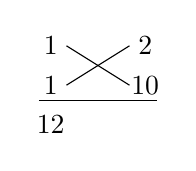
\begin{tikzpicture}
				% Numbers
				\node at (0, 1) {1};
				\node at (1.2, 1) {2};
				
				\node at (0, 0.5) {1};
				\node at (1.2, 0.5) {10};
				
				\node at (0.6, 0.3) {\rule{1.5cm}{0.4pt}}; % horizontal line
				
				\node at (0, 0) {12};
				
				% Cross lines
				\draw (0.2,1) -- (1,0.5); % from 1 (top left) to 10
				\draw (0.2,0.5) -- (1,1); % from 1 (bottom left) to 2
			\end{tikzpicture}
			
			%2
			\item 原式$=(x-2)(x-10)$.\\
			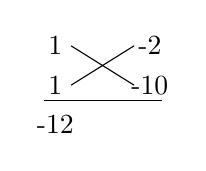
\begin{tikzpicture}
				% Numbers
				\node at (0, 1) {1};
				\node at (1.2, 1) {-2};
				
				\node at (0, 0.5) {1};
				\node at (1.2, 0.5) {-10};
				
				\node at (0.6, 0.3) {\rule{1.5cm}{0.4pt}}; % horizontal line
				
				\node at (0, 0) {-12};
				
				% Cross lines
				\draw (0.2,1) -- (1,0.5); % from 1 (top left) to 10
				\draw (0.2,0.5) -- (1,1); % from 1 (bottom left) to 2
			\end{tikzpicture}
			
			%3
			\item 原式$=(x+1)(x-5)$.\\
			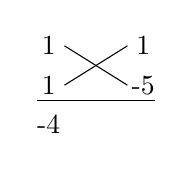
\begin{tikzpicture}
				% Numbers
				\node at (0, 1) {1};
				\node at (1.2, 1) {1};
				
				\node at (0, 0.5) {1};
				\node at (1.2, 0.5) {-5};
				
				\node at (0.6, 0.3) {\rule{1.5cm}{0.4pt}}; % horizontal line
				
				\node at (0, 0) {-4};
				
				% Cross lines
				\draw (0.2,1) -- (1,0.5); % from 1 (top left) to 10
				\draw (0.2,0.5) -- (1,1); % from 1 (bottom left) to 2
			\end{tikzpicture}
			
			%4
			\item 原式$=(x+2)(x-11)$.\\
			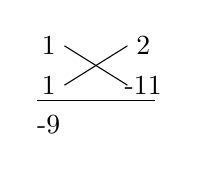
\begin{tikzpicture}
				% Numbers
				\node at (0, 1) {1};
				\node at (1.2, 1) {2};
				
				\node at (0, 0.5) {1};
				\node at (1.2, 0.5) {-11};
				
				\node at (0.6, 0.3) {\rule{1.5cm}{0.4pt}}; % horizontal line
				
				\node at (0, 0) {-9};
				
				% Cross lines
				\draw (0.2,1) -- (1,0.5); % from 1 (top left) to 10
				\draw (0.2,0.5) -- (1,1); % from 1 (bottom left) to 2
			\end{tikzpicture}
			
			%5
			\item 原式$=(3x-5y)(4x+3y)$.\\
			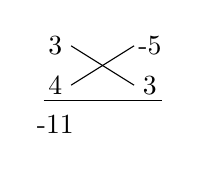
\begin{tikzpicture}
				% Numbers
				\node at (0, 1) {3};
				\node at (1.2, 1) {-5};
				
				\node at (0, 0.5) {4};
				\node at (1.2, 0.5) {3};
				
				\node at (0.6, 0.3) {\rule{1.5cm}{0.4pt}}; % horizontal line
				
				\node at (0, 0) {-11};
				
				% Cross lines
				\draw (0.2,1) -- (1,0.5); % from 1 (top left) to 10
				\draw (0.2,0.5) -- (1,1); % from 1 (bottom left) to 2
			\end{tikzpicture}
			
			%6
			\item 原式$=(2x-3)(3x-2)$.\\
			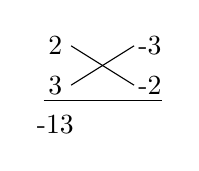
\begin{tikzpicture}
				% Numbers
				\node at (0, 1) {2};
				\node at (1.2, 1) {-3};
				
				\node at (0, 0.5) {3};
				\node at (1.2, 0.5) {-2};
				
				\node at (0.6, 0.3) {\rule{1.5cm}{0.4pt}}; % horizontal line
				
				\node at (0, 0) {-13};
				
				% Cross lines
				\draw (0.2,1) -- (1,0.5); % from 1 (top left) to 10
				\draw (0.2,0.5) -- (1,1); % from 1 (bottom left) to 2
			\end{tikzpicture}
			
			%7
			\item 原式$=(2x+1)(x+3)$.\\
			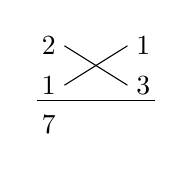
\begin{tikzpicture}
				% Numbers
				\node at (0, 1) {2};
				\node at (1.2, 1) {1};
				
				\node at (0, 0.5) {1};
				\node at (1.2, 0.5) {3};
				
				\node at (0.6, 0.3) {\rule{1.5cm}{0.4pt}}; % horizontal line
				
				\node at (0, 0) {7};
				
				% Cross lines
				\draw (0.2,1) -- (1,0.5); % from 1 (top left) to 10
				\draw (0.2,0.5) -- (1,1); % from 1 (bottom left) to 2
			\end{tikzpicture}
			
			%8
			\item 原式$=(x-1)(2x-3)$.\\
			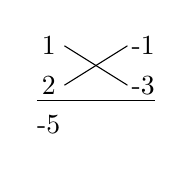
\begin{tikzpicture}
				% Numbers
				\node at (0, 1) {1};
				\node at (1.2, 1) {-1};
				
				\node at (0, 0.5) {2};
				\node at (1.2, 0.5) {-3};
				
				\node at (0.6, 0.3) {\rule{1.5cm}{0.4pt}}; % horizontal line
				
				\node at (0, 0) {-5};
				
				% Cross lines
				\draw (0.2,1) -- (1,0.5); % from 1 (top left) to 10
				\draw (0.2,0.5) -- (1,1); % from 1 (bottom left) to 2
			\end{tikzpicture}
			
			%9
			\item 原式$=x^2-20xy+64y^2\\=(x-4y)(x-16y)$.\\
			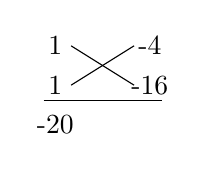
\begin{tikzpicture}
				% Numbers
				\node at (0, 1) {1};
				\node at (1.2, 1) {-4};
				
				\node at (0, 0.5) {1};
				\node at (1.2, 0.5) {-16};
				
				\node at (0.6, 0.3) {\rule{1.5cm}{0.4pt}}; % horizontal line
				
				\node at (0, 0) {-20};
				
				% Cross lines
				\draw (0.2,1) -- (1,0.5); % from 1 (top left) to 10
				\draw (0.2,0.5) -- (1,1); % from 1 (bottom left) to 2
			\end{tikzpicture}
			
			%10
			\item 原式$=-(x^2-x-56)\\=-(x+7)(x-8)$.\\
			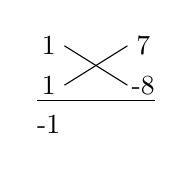
\begin{tikzpicture}
				% Numbers
				\node at (0, 1) {1};
				\node at (1.2, 1) {7};
				
				\node at (0, 0.5) {1};
				\node at (1.2, 0.5) {-8};
				
				\node at (0.6, 0.3) {\rule{1.5cm}{0.4pt}}; % horizontal line
				
				\node at (0, 0) {-1};
				
				% Cross lines
				\draw (0.2,1) -- (1,0.5); % from 1 (top left) to 10
				\draw (0.2,0.5) -- (1,1); % from 1 (bottom left) to 2
			\end{tikzpicture}
			
			%11
			\item 原式$=[x-(b+c)][(b+c)x-bc]\\=(x-b-c)(bx+cx-bc)$.\\
			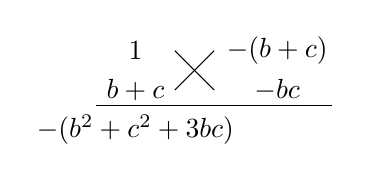
\begin{tikzpicture}
				% Numbers
				\node at (0, 1) {1};
				\node at (1.8, 1) {$-(b+c)$};
				
				\node at (0, 0.5) {$b+c$};
				\node at (1.8, 0.5) {$-bc$};
				
				\node at (1, 0.3) {\rule{3cm}{0.4pt}}; % horizontal line
				
				\node at (0, 0) {$-(b^2+c^2+3bc)$};
				
				% Cross lines
				\draw (0.5,1) -- (1,0.5); % from 1 (top left) to 10
				\draw (0.5,0.5) -- (1,1); % from 1 (bottom left) to 2
			\end{tikzpicture}
			
			
			%12
			\item 原式$=(ax+a+1)(ax+x+a)$.\\
			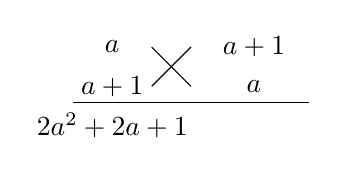
\begin{tikzpicture}
				% Numbers
				\node at (0, 1) {$a$};
				\node at (1.8, 1) {$a+1$};
				
				\node at (0, 0.5) {$a+1$};
				\node at (1.8, 0.5) {$a$};
				
				\node at (1, 0.3) {\rule{3cm}{0.4pt}}; % horizontal line
				
				\node at (0, 0) {$2a^2+2a+1$};
				
				% Cross lines
				\draw (0.5,1) -- (1,0.5); % from 1 (top left) to 10
				\draw (0.5,0.5) -- (1,1); % from 1 (bottom left) to 2
			\end{tikzpicture}
		\end{multicols}
	\end{enumerate}
}		
\end{document}
